\documentclass[11pt]{article}

% --- Packages ---
\usepackage[margin=1in]{geometry}
\usepackage{amsmath,amssymb}
\usepackage{graphicx}
\usepackage[colorlinks=true,linkcolor=blue,citecolor=blue,urlcolor=blue]{hyperref}
\usepackage{natbib}
\usepackage{booktabs}
\usepackage{multirow}
\usepackage{caption}
\usepackage{subcaption}
\usepackage{algorithm}
\usepackage{algpseudocode}
\usepackage{xcolor}

% --- Metadata ---
\title{\textbf{hemosim}: A Reproducible, Calibrated, Clinically-Safe\\
Simulation Infrastructure for Reinforcement-Learning Research\\
in Hemostasis and Anticoagulation Management}
\author{
  Hass Dhia\\
  Smart Technology Investments Research Institute\\
  \texttt{hass@smarttechinvest.com}
}
\date{April 2026 --- v2.0}

\begin{document}

\maketitle

% ============================================================================
% SECTION 1: ABSTRACT
% ============================================================================
\begin{abstract}
Anticoagulation therapy affects millions of patients worldwide, yet dosing errors remain a leading contributor to preventable inpatient harm. Reinforcement learning (RL) has been proposed as a tool for individualized anticoagulant dosing since at least the deep-RL work of \citet{nemati2016}, but the absence of a shared, reproducible, clinically calibrated simulation benchmark has limited the field to ad-hoc environments that cannot be independently re-run or compared. We introduce \texttt{hemosim} v2, a simulation infrastructure explicitly positioned as Phase~1 of a five-phase clinical translation pathway for RL anticoagulation policies. \texttt{hemosim} contributes: (a)~four Gymnasium-compatible environments grounded in published PK/PD models --- warfarin titration, unfractionated heparin infusion, DOAC management, and DIC; (b)~a POMDP reformulation with explicit lab ordering as an action, per-lab turnaround times (TATs), and analytical variability, replacing the oracle-lab assumption that clinicians identified as the single largest deviation from bedside reality; (c)~mechanistic coupling to a reduced coagulation cascade ODE in the DIC environment; (d)~clinical-outcome metrics (Rosendaal time-in-therapeutic-range, ISTH major bleeding, thromboembolic event aggregation, Warkentin 4T HIT score, and an explicitly-flagged mortality proxy) emitted by every environment; (e)~published-data calibration with a normalized RMSE of 0.0013 on warfarin against Hamberg \citep{hamberg2007} and IWPC \citep{iwpc2009} targets, and honest residuals on the Nemati~2016 TTR target on heparin that motivate the POMDP reformulation; (f)~a clinical decision support harness with a rule-based safety layer enforcing absolute dose caps, contraindication checks, and uncertainty-aware deferral; (g)~a SPIRIT~2013-compliant silent-deployment observational trial protocol; and (h)~an extensible benchmark baselines suite that includes a faithful reimplementation of the \citet{nemati2016} DQN heparin policy. We explicitly disclose that end-to-end PPO policy training on the calibrated environment is Phase~2 work, deferred to a companion paper contingent on individual-patient MIMIC-IV calibration. The present paper reports only reproducible baseline results (clinical-guideline agents and random controls) on held-out seed pools, calibration residuals, and infrastructure validation. All numbers tie back to commands that anyone with the repository can re-run. \texttt{hemosim} is available under the MIT license (\texttt{pip install hemosim}), ships 142 unit and integration tests, and is designed to be the shared substrate on which future work --- including \citet{nemati2016} replication and Phase~3 silent deployment --- can be measured.
\end{abstract}

% ============================================================================
% SECTION 2: INTRODUCTION
% ============================================================================
\section{Introduction}
\label{sec:introduction}

Anticoagulation therapy is among the most common and consequential pharmacological interventions in modern medicine. Warfarin remains the most widely prescribed oral anticoagulant globally despite the emergence of direct oral anticoagulants (DOACs), and unfractionated heparin is the standard parenteral anticoagulant for acute thrombotic events \citep{hirsh2001}. Together, anticoagulants are prescribed to tens of millions of patients for conditions including atrial fibrillation, venous thromboembolism, mechanical heart valves, and disseminated intravascular coagulation (DIC).

The clinical challenge of anticoagulation lies in its narrow therapeutic window. Insufficient anticoagulation permits thromboembolic events --- stroke, pulmonary embolism, deep vein thrombosis --- while excessive anticoagulation causes hemorrhage, which can be fatal. Warfarin's therapeutic index is notoriously narrow: the international normalized ratio (INR) target range of 2.0--3.0 leaves little margin for error, and patient response varies dramatically based on genetics (CYP2C9, VKORC1), diet, concomitant medications, and acute illness \citep{iwpc2009, johnson2017}. Heparin dosing faces analogous challenges with activated partial thromboplastin time (aPTT) targets of 60--100 seconds \citep{raschke1993}. DOACs, while requiring less routine monitoring, demand drug and dose selection based on renal function, stroke risk, and bleeding risk \citep{connolly2009, patel2011, granger2011}. DIC represents the most complex scenario: simultaneous hemorrhage and thrombosis requiring coordinated multi-component therapy \citep{levi1999, levi2009}.

These characteristics make anticoagulation management a natural candidate for reinforcement learning (RL). The problem is inherently sequential: a clinician \emph{orders labs}, \emph{waits} for results that arrive with delay and analytical noise, \emph{observes} the returned values, \emph{selects} an action (dose, drug), and the patient transitions to a new state determined by pharmacokinetics and pharmacodynamics. The delayed, noisy, action-conditioned nature of the observation process further aligns with the formulation of partially observable sequential decision-making under uncertainty.

Prior work has demonstrated the potential of RL for clinical dosing. \citet{nemati2016} applied deep Q-learning to heparin dosing from MIMIC-II retrospective data, reporting that learned policies improved time-in-therapeutic-range relative to the observed Raschke nomogram baseline. \citet{raghu2017} applied continuous-state RL to sepsis management, and \citet{komorowski2018} published the ``AI Clinician'' for sepsis treatment in \emph{Nature Medicine}. \citet{anzabizadeh2023} and \citet{tosca2024} systematically reviewed RL approaches for warfarin and clinical pharmacology respectively. However, a structural limitation pervades this literature: each study constructs an ad-hoc simulation environment that cannot be reproduced or directly compared across research groups. The lack of standardized benchmarks has been called out by reviewers of the field as the single largest methodological obstacle to scientific comparison \citep{ghassemi2018}.

In parallel, the clinical community has consistently raised three concerns about RL anticoagulation papers: (i)~the simulated environments expose oracle labs at every timestep rather than the delayed, noisy labs a bedside clinician must order; (ii)~reported policy improvements are not accompanied by re-runnable results that a pharmacist or clinical statistician can verify; and (iii)~the clinical utility is not stated in the outcome metrics that govern regulatory and payor review (time-in-therapeutic-range, ISTH major bleeding, thromboembolic events, HIT).

\texttt{hemosim} v2 addresses each of these gaps directly. We contribute:
\begin{enumerate}
  \item Four Gymnasium-compatible environments spanning the major anticoagulation modalities, each grounded in published PK/PD models.
  \item A POMDP reformulation (\S\ref{sec:pomdp}) with explicit lab-ordering actions, per-lab turnaround times, and analytical variability drawn from the clinical-chemistry literature \citep{bowen2016, lippi2012, whitehead2020}.
  \item Mechanistic coupling of the reduced Hockin--Mann coagulation cascade \citep{hockin2002} to the DIC environment (\S\ref{sec:cascade}), replacing a prior flat-state approximation.
  \item A published-data calibration harness (\S\ref{sec:calibration}) that fits PK/PD parameters against IWPC, Hamberg, Raschke, Hirsh, Nemati, RE-LY, ROCKET-AF, and ARISTOTLE cohort summaries, with documented residuals.
  \item Clinical-outcome metrics (\S\ref{sec:metrics}): Rosendaal TTR \citep{rosendaal1993}, ISTH major bleeding \citep{schulman2005iostroke}, a thromboembolic event aggregator, Warkentin 4T HIT scoring \citep{warkentin2003, lo2006}, and a composite mortality proxy (explicitly flagged as a proxy).
  \item A clinical decision support (CDS) harness with a rule-based safety layer (\S\ref{sec:dss}) that enforces absolute dose caps, contraindication checks, and uncertainty-aware deferral, following \citet{holbrook2012} and standard antithrombotic stewardship practice.
  \item A SPIRIT~2013-compliant silent-deployment observational trial protocol (\S\ref{sec:protocol}) that specifies how a locked policy would be evaluated against usual care without influencing patient management.
  \item An extensible baselines suite, including a faithful reimplementation of the \citet{nemati2016} DQN heparin policy as a benchmark row, a Gage pharmacogenetic warfarin baseline, an anti-Xa-guided heparin baseline, and the standard Raschke and IWPC baselines.
  \item Full reproducibility infrastructure (\S\ref{sec:reproducibility}): disjoint train/eval seed pools, a one-command \texttt{./scripts/reproduce.sh} path, and a reference \texttt{EXPECTED\_RESULTS.json} with a 5\%-tolerance comparison check.
\end{enumerate}

\paragraph{Scope and limitations of this paper.}
This paper introduces the simulation infrastructure and reports its validation against published data. It does \emph{not} report end-to-end training results for a Proximal Policy Optimization (PPO) or other RL policy on the calibrated environment. PPO policy training against the POMDP-reformulated, calibration-fitted environment is the subject of a forthcoming companion paper contingent on individual-patient MIMIC-IV calibration; we call this Phase~2. The rationale for separating infrastructure and policy into two papers is scientific: cohort-level calibration of PK/PD parameters against summary statistics is a necessary but insufficient condition for training a bedside-ready RL policy. Individual-level calibration against MIMIC-IV \citep{johnson2023mimic4} aPTT and INR trajectories is Phase~2 work, and policy claims are honest only once that calibration is complete. The present paper reports reproducible baseline numbers (clinical-guideline agents and random controls on held-out seed pools), calibration residuals, and infrastructure correctness. No end-to-end RL policy claim is made in \S\ref{sec:results}.

% ============================================================================
% SECTION 3: RELATED WORK
% ============================================================================
\section{Related Work}
\label{sec:related_work}

The development of \texttt{hemosim} draws on three intersecting literatures: mathematical models of coagulation and anticoagulant pharmacology, clinical dosing guidelines, and reinforcement learning for healthcare. Because reviewers of v0.1 specifically asked for an explicit, one-by-one comparison between \texttt{hemosim} and each prior RL-for-clinical-dosing effort, we provide that comparison here.

\paragraph{Mathematical models of coagulation.}
\citet{hockin2002} developed the foundational 34-species ordinary differential equation (ODE) model of tissue-factor-initiated coagulation. \citet{chatterjee2010} extended systems-biology approaches to thrombin generation in whole blood. \citet{wajima2009} proposed a comprehensive humoral-coagulation-network model suitable for pharmacological simulation. \citet{danforth2009} quantified uncertainty propagation and \citet{brummelziedins2013} reviewed thrombin-generation models in disease-risk contexts. These models provide the mechanistic foundation for realistic simulation but are computationally expensive for RL training, motivating the reduced-order formulation used in \texttt{hemosim} (\S\ref{sec:models}).

\paragraph{Warfarin pharmacogenomics.}
The International Warfarin Pharmacogenetics Consortium \citep{iwpc2009} established the landmark dosing algorithm incorporating CYP2C9 and VKORC1 genotypes. \citet{hamberg2007, hamberg2010} developed the population PK--PD model relating warfarin pharmacokinetics to INR response. \citet{gage2008} produced a competing pharmacogenomic dosing algorithm. CPIC codified these findings into practice guidelines \citep{johnson2017}. These models and algorithms serve both as the mechanistic basis for our warfarin environment and as baseline agents.

\paragraph{Heparin dosing.}
\citet{raschke1993} established the weight-based heparin nomogram that remains the standard of care. \citet{hirsh2001} provided comprehensive guidelines for heparin therapy. \citet{holbrook2012} represent the most recent ACCP guideline for antithrombotic therapy. These sources form the clinical baseline in our heparin environment and the rule-base in the safety layer (\S\ref{sec:dss}).

\paragraph{Laboratory turnaround and variability.}
Laboratory TATs and analytical variability are the substrate of the POMDP reformulation. \citet{bowen2016} and \citet{whitehead2020} document pre-analytical variability in coagulation and hematology assays. \citet{lippi2012} reviews milestones and remaining challenges in coagulation testing. \citet{vandenbesselaar2010} documents inter-laboratory reproducibility of INR. These sources are the basis for the per-lab TAT and CV specifications in Table~\ref{tab:lab_panel}.

\paragraph{Direct oral anticoagulants.}
Three landmark trials established DOACs for atrial fibrillation: RE-LY \citep{connolly2009}, ROCKET-AF \citep{patel2011}, and ARISTOTLE \citep{granger2011}. \citet{mueck2007} published rivaroxaban population PK. Stroke and bleeding risk stratification use CHA$_2$DS$_2$-VASc \citep{lip2010} and HAS-BLED \citep{pisters2010}. Published event rates from these trials are calibration targets in \S\ref{sec:calibration}.

\paragraph{Disseminated intravascular coagulation.}
\citet{taylor2001} developed the ISTH DIC scoring system. \citet{levi1999, levi2009} review pathophysiology and management. The ISTH score serves as both the primary state variable and a reward component in the DIC environment.

\paragraph{Heparin-induced thrombocytopenia.}
\citet{warkentin2003} and \citet{lo2006} developed the 4T scoring system. \citet{greinacher2019} reviews autoimmune HIT. Implementing a 4T score emitter (\S\ref{sec:metrics}) allows the environment to report HIT risk on every episode rather than relying on downstream code to re-derive it.

\subsection{Reinforcement learning for clinical dosing: explicit comparisons}

\paragraph{\citet{nemati2016} --- Deep RL for heparin dosing from MIMIC-II.}
The foundational RL anticoagulation paper. Nemati, Ghassemi, and Clifford trained a DQN on a retrospective MIMIC-II heparin cohort and reported improved time-in-therapeutic-range relative to the observed Raschke nomogram baseline. What \citet{nemati2016} could \emph{not} do, by design, is release a shared simulation environment: the MIMIC-II data used were institutionally held, and the reconstruction of the state transition was tied to that specific cohort. \texttt{hemosim} explicitly targets the reproducibility gap: the environment is released pip-installable, the Raschke baseline is reimplemented as a shared reference, and \citet{nemati2016}'s DQN architecture is reimplemented (\texttt{src/hemosim/agents/baselines\_extended.py::NematiDQN2016Baseline}) so that its performance on the shared environment can be measured alongside the other baselines. The calibration section (\S\ref{sec:calibration}) treats the Nemati~2016 TTR on the Raschke nomogram (0.55) as a published target, and our honest residual of $-0.175$ at the cohort level motivates exactly the POMDP reformulation described in \S\ref{sec:pomdp}.

\paragraph{\citet{ghassemi2018} and Ghassemi 2017 --- MIMIC-based clinical RL and inverse RL for sepsis.}
Ghassemi's group has produced a series of papers using MIMIC data for clinical RL and inverse-RL for sepsis management. The methodological parallel to \texttt{hemosim} is the insight that clinician decisions are demonstrations of a policy under partial observability, not of a full-information optimal controller. The structural difference is that \texttt{hemosim} publishes the environment rather than the retrospective dataset, enabling prospective comparison across algorithms.

\paragraph{\citet{komorowski2018} --- AI Clinician for sepsis in \emph{Nature Medicine}.}
The ``AI Clinician'' paper set the regulatory-visibility benchmark for RL in critical care, using discretized state-action Q-learning on MIMIC-III and eICU data to derive a sepsis resuscitation policy. Two specific methodological parallels motivated our silent-deployment protocol (\S\ref{sec:protocol}): (a)~Komorowski et al.'s counterfactual-value framework for evaluating a learned policy against clinician-observed actions, and (b)~the emphasis on a pre-registered, externally validated endpoint before any prospective use. \texttt{hemosim}'s silent-deployment protocol adapts both, with Rosendaal TTR as the primary endpoint and a DSMB bleed-proximity stopping rule.

\paragraph{\citet{raghu2017} --- Continuous-state RL for sepsis treatment.}
Raghu et al. extended the AI-Clinician line of work to continuous state representations using neural-network Q-functions on MIMIC sepsis data. Their 2017 paper is the reference point for continuous-state clinical RL; \texttt{hemosim}'s Gymnasium continuous observation spaces (\S\ref{sec:environments}) match that formulation.

\paragraph{\texttt{simglucose} --- open-source T1D simulator precedent.}
The \texttt{simglucose} package \citep{simglucose} wraps the FDA-accepted UVa/Padova Type-1 Diabetes simulator in the OpenAI~Gym interface, enabling a generation of closed-loop insulin-delivery RL research to use a shared benchmark. \texttt{hemosim} is deliberately patterned on this precedent and extends it to anticoagulation: a pip-installable, Gymnasium-compatible environment with a rigorously calibrated mechanistic substrate and documented residuals.

\paragraph{\citet{kuo2022} --- Health Gym.}
The Health Gym work by Kuo et al. introduced synthetic datasets for RL in sepsis and other critical-care domains using a generative-model approach. The methodological contrast is that Health Gym emphasizes synthetic retrospective cohorts, whereas \texttt{hemosim} emphasizes mechanistic simulation of PK/PD with published-data calibration. We view the two as complementary: \texttt{hemosim} suits problems where the pharmacological substrate is well-characterized; Health Gym suits problems where the evolution of disease state is not reducible to a small ODE.

\paragraph{\citet{anzabizadeh2023} and \citet{tosca2024}.}
Two recent reviews. \citet{anzabizadeh2023} systematically reviewed RL approaches for warfarin dosing, identifying heterogeneity in problem formulation, state representation, and reward design as the primary obstacles to scientific comparison --- exactly the gap \texttt{hemosim} targets. \citet{tosca2024} surveyed RL applications across clinical pharmacology, including dosing, treatment scheduling, and adaptive clinical trials.

\paragraph{The gap, restated.}
No prior work ships a Gymnasium-compatible, PK/PD-calibrated, POMDP-correct anticoagulation environment with published residuals, clinical-outcome metrics, a rule-based safety layer, a silent-deployment protocol, and a reimplementation of the seminal \citet{nemati2016} DQN as a shared baseline. \texttt{hemosim} is that package.

% ============================================================================
% SECTION 4: SYSTEM ARCHITECTURE
% ============================================================================
\section{System Architecture}
\label{sec:architecture}

\texttt{hemosim} is structured as a standard Python package using the \texttt{src} layout convention:

\begin{verbatim}
hemosim/
  src/hemosim/
    envs/                   # Gymnasium environments
      warfarin_dosing.py
      heparin_infusion.py
      heparin_infusion_pomdp.py     # POMDP reformulation (ISC-5)
      pomdp.py                       # base POMDP + LabOrderQueue
      doac_management.py
      dic_management.py
    models/                 # PK/PD and coagulation models
      coagulation.py        # Hockin-Mann reduced ODE
      warfarin_pkpd.py
      heparin_pkpd.py
      doac_pkpd.py
      patient.py
    metrics/                # Clinical-outcome metrics (ISC-4)
      clinical.py
    clinical/               # CDS harness + safety layer (ISC-10+11)
      dss.py
      safety.py
    agents/                 # RL agents and baselines
      baselines.py                  # Clinical protocol agents
      baselines_extended.py         # Anti-Xa, Gage, Nemati DQN 2016
      ppo.py                         # PPO training wrapper
    benchmarks/             # Evaluation harness
      runner.py
    validation/             # MIMIC-IV calibration scaffold
      mimic_calibration.py
    reproducibility.py       # Seed pools (train vs held-out)
  scripts/
    reproduce.sh                    # one-command repro
    generate_results.py             # baselines on held-out seeds
    run_published_calibration.py    # Hamberg/IWPC/Raschke/Hirsh/Nemati fit
    run_mimic_calibration.py        # MIMIC-IV scaffold
    train_nemati_dqn.py             # reimplementation of Nemati 2016
  tests/                     # 142 unit and integration tests
  results/                   # JSON artifacts + EXPECTED_RESULTS.json
  figures/
  paper/                     # This manuscript + silent-deployment protocol
\end{verbatim}

\subsection{Model hierarchy}

The architecture follows a four-layer hierarchy:

\begin{enumerate}
  \item \textbf{PK/PD models} (\texttt{models/}): Mechanistic ODE models that simulate drug pharmacokinetics and pharmacodynamics. These models accept drug doses and patient parameters, integrate ODEs using \texttt{scipy.integrate.solve\_ivp}, and return updated physiological state (INR, aPTT, drug concentrations, coagulation species).
  \item \textbf{Gymnasium environments} (\texttt{envs/}): Standard \texttt{Env} subclasses that wrap PK/PD models with observation spaces, action spaces (including lab-ordering actions in the POMDP formulation), reward functions, and termination conditions. Each environment is registered with Gymnasium and instantiated via \texttt{gymnasium.make("hemosim/WarfarinDosing-v0")}.
  \item \textbf{Clinical-outcome metrics} (\texttt{metrics/clinical.py}): Rosendaal TTR, ISTH major bleeding, thromboembolic event aggregator, Warkentin 4T HIT scoring, and a composite mortality proxy. Every environment emits these values in the \texttt{info} dict of each step.
  \item \textbf{Clinical decision support harness and safety layer} (\texttt{clinical/}): A FHIR-shaped \texttt{PatientSnapshot} input, a \texttt{DosingRecommendation} output with uncertainty intervals and saliency, and a \texttt{SafeDSS} wrapper that applies absolute dose caps, contraindication checks, and uncertainty-aware deferral before a recommendation is surfaced to a consumer.
  \item \textbf{Agents and baselines} (\texttt{agents/}): Clinical-guideline agents (IWPC warfarin, Raschke heparin, anti-Xa heparin, Gage warfarin, ISTH-guided DIC, guideline DOAC) plus a reimplemented Nemati~2016 DQN as a reference. PPO wrappers from Stable-Baselines3 \citep{stablebaselines3, schulman2017ppo} are included but training results are \emph{not} reported in this paper (see \S\ref{sec:introduction} and \S\ref{sec:discussion}).
\end{enumerate}

\subsection{Patient generation}

The \texttt{PatientGenerator} class produces stochastic patient profiles with pharmacogenomic variability. For warfarin patients, this includes CYP2C9 genotype (six allele combinations: \texttt{*1/*1}, \texttt{*1/*2}, \texttt{*1/*3}, \texttt{*2/*2}, \texttt{*2/*3}, \texttt{*3/*3}) and VKORC1 genotype (GG, GA, AA), sampled from published population frequencies. Patient demographics (age, weight, renal function) are drawn from distributions calibrated to clinical-study populations. Each environment's \texttt{reset()} method generates a new patient from a seed, ensuring episode diversity during training and deterministic reproducibility given a fixed seed.

\subsection{Difficulty tiers}

Each environment supports three difficulty tiers:
\begin{itemize}
  \item \textbf{Easy}: Stable patients, reduced variability, no complications. Suitable for algorithm development and debugging.
  \item \textbf{Medium}: Full pharmacogenomic variability, standard clinical complexity. The default tier for calibration and reported baseline results.
  \item \textbf{Hard}: Additional complications (drug interactions, acute illness, perioperative management, concurrent hemorrhage and thrombosis). Designed for curriculum-learning research.
\end{itemize}

% ============================================================================
% SECTION 5: ENVIRONMENT DESIGN
% ============================================================================
\section{Environment Design}
\label{sec:environments}

This section details the observation space, action space, reward function, and termination conditions for each of the four fully-observable environments. The POMDP reformulation of the heparin environment is described separately in \S\ref{sec:pomdp}.

\subsection{Warfarin Dose Titration (\texttt{hemosim/WarfarinDosing-v0})}

\paragraph{Task.} Titrate daily warfarin dose over 90 days to maintain INR within 2.0--3.0, accounting for patient-specific CYP2C9 and VKORC1 pharmacogenomics.

\paragraph{Observation space.} $\mathbb{R}^{8}$, normalized to $[0,1]$: INR, S-warfarin, R-warfarin plasma concentrations, age, weight, CYP2C9 genotype (ordinal 0--5), VKORC1 genotype (ordinal 0--2), days on therapy.

\paragraph{Action space.} $\mathbb{R}^{1}$, continuous $[0,1]$ mapped to $[0,15]$~mg warfarin daily dose.

\paragraph{Reward function.}
\begin{equation}
  r_t = -|{\rm INR}_t - 2.5| + 0.5 \cdot \mathbf{1}[2.0 \leq {\rm INR}_t \leq 3.0] - 10 \cdot \mathbf{1}[{\rm INR}_t > 4.0] - 5 \cdot \mathbf{1}[{\rm INR}_t < 1.5]
  \label{eq:warfarin_reward}
\end{equation}
with additional termination penalties of $-20$ for INR $> 6.0$ and $-10$ for INR $< 1.0$.

\paragraph{Termination.} Episode terminates after 90 days or if INR exceeds 6.0 or falls below 1.0.

\subsection{Heparin Infusion (\texttt{hemosim/HeparinInfusion-v0})}

\paragraph{Task.} Manage continuous unfractionated heparin infusion over 120~hours (5~days) with decisions every 6~hours, maintaining aPTT of 60--100~s.

\paragraph{Observation space.} $\mathbb{R}^{6}$: aPTT, heparin concentration, weight, renal function, platelet count, hours since therapy start. (The POMDP reformulation replaces this fully-observable oracle view with a delayed, noisy, action-ordered lab buffer; see \S\ref{sec:pomdp}.)

\paragraph{Action space.} $\mathbb{R}^{2}$: infusion rate $[0, 2500]$~U/hr, bolus flag (triggers 80~U/kg).

\paragraph{Reward function.}
\begin{equation}
  r_t = -\tfrac{|{\rm aPTT}_t - 75|}{30} + 0.5 \cdot \mathbf{1}[60 \leq {\rm aPTT}_t \leq 100] - 5 \cdot \mathbf{1}[{\rm aPTT}_t > 120] - 3 \cdot \mathbf{1}[{\rm aPTT}_t < 40]
  \label{eq:heparin_reward}
\end{equation}
with termination penalties of $-20$ for platelet count $< 50{,}000$ and $-15$ for aPTT $> 150$.

\subsection{DOAC Management (\texttt{hemosim/DOACManagement-v0})}

\paragraph{Task.} Select and dose DOACs for atrial fibrillation over 365~days with monthly decisions, balancing stroke prevention and bleeding risk.

\paragraph{Observation space.} $\mathbb{R}^{8}$: drug concentration, CrCl, age, weight, CHA$_2$DS$_2$-VASc \citep{lip2010}, HAS-BLED \citep{pisters2010}, days on therapy, current drug.

\paragraph{Action space.} \texttt{MultiDiscrete([3, 3])}: drug $\in \{$rivaroxaban, dabigatran, apixaban$\}$; dose $\in \{$low, standard, high$\}$.

\paragraph{Reward function.}
\begin{equation}
  r_t = 1.0 - 20 \cdot \mathbf{1}[\text{stroke}] - 10 \cdot \mathbf{1}[\text{major bleed}] - 5 \cdot \mathbf{1}[\text{drug switch}] + 0.5 \cdot \mathbf{1}[\text{dose appropriate for CrCl}]
  \label{eq:doac_reward}
\end{equation}
Event probabilities are derived from RE-LY \citep{connolly2009}, ROCKET-AF \citep{patel2011}, and ARISTOTLE \citep{granger2011}.

\subsection{DIC Management (\texttt{hemosim/DICManagement-v0})}

\paragraph{Task.} Manage DIC over 168~hours (7~days) with treatment decisions every 4~hours, coordinating blood products and heparin against simultaneous hemorrhage and thrombosis.

\paragraph{Observation space.} $\mathbb{R}^{8}$: ISTH DIC score \citep{taylor2001}, platelet count, fibrinogen, PT prolongation, D-dimer, organ function, hours elapsed, hemorrhage severity.

\paragraph{Action space.} \texttt{MultiDiscrete([4, 4, 3, 3])}: platelet transfusion $\in \{0, 1, 2, 4\}$ units, FFP $\in \{0, 2, 4, 6\}$ units, cryoprecipitate $\in \{0, 5, 10\}$ units, heparin $\in \{$none, 500, 1000$\}$~U/hr.

\paragraph{Reward function.}
\begin{equation}
  r_t = -S_t^{\rm DIC} + 2 \cdot \mathbf{1}[\Delta S < 0] - 5 \cdot \mathbf{1}[h_t > 0.5] - c_{\rm tx} - 3 \cdot \mathbf{1}[\text{heparin} \wedge \text{plt} < 50\text{k}]
  \label{eq:dic_reward}
\end{equation}
where $S_t^{\rm DIC}$ is the ISTH DIC score, $\Delta S$ is the change from the previous step, $h_t$ is hemorrhage severity, and $c_{\rm tx}$ is a resource-utilization cost proportional to transfusion volume.

% ============================================================================
% SECTION 6: SIGNAL AND PHYSICS MODELS
% ============================================================================
\section{Signal and Physics Models}
\label{sec:models}

The environments are grounded in mechanistic models from the coagulation and clinical pharmacology literature. This section describes each model, its relationship to the gold-standard formulation, and the simplifications made for computational tractability.

\subsection{Coagulation cascade: 8-state reduced ODE}

The foundation of \texttt{hemosim}'s physiological modeling is a reduced coagulation cascade model simplified from the \citet{hockin2002} 34-species ODE. The full Hockin--Mann model tracks 34 biochemical species through initiation, amplification, and propagation, requiring stiff ODE integration that is prohibitively expensive for RL training. Our 8-state reduced system retains the key dynamical features while achieving two orders of magnitude speedup:
\begin{align}
  \frac{d[\text{TF:VIIa}]}{dt} &= k_1 - k_2 [\text{TF:VIIa}] \label{eq:coag_tfviia} \\
  \frac{d[\text{Xa}]}{dt} &= k_3 [\text{TF:VIIa}] - k_4 [\text{Xa}] \\
  \frac{d[\text{Va}]}{dt} &= k_5 [\text{IIa}] - k_6 [\text{Va}] \\
  \frac{d[\text{IIa}]}{dt} &= k_7 [\text{Xa}][\text{Va}][\text{Pro}] - k_8 [\text{IIa}] - k_9 [\text{AT\text{-}III}][\text{IIa}] \\
  \frac{d[\text{Fgn}]}{dt} &= -k_{10} [\text{IIa}][\text{Fgn}] \\
  \frac{d[\text{Fbn}]}{dt} &= k_{10} [\text{IIa}][\text{Fgn}] \\
  \frac{d[\text{AT\text{-}III}_b]}{dt} &= k_9 ([\text{AT\text{-}III}]_0 - [\text{AT\text{-}III}_b])[\text{IIa}] \\
  \frac{d[\text{Plt}_a]}{dt} &= k_{11} [\text{IIa}](1 - [\text{Plt}_a]) - k_{12} [\text{Plt}_a]
\end{align}
This captures TF-initiated activation, the thrombin positive-feedback loop, fibrin formation, antithrombin inhibition, and platelet activation.

\subsection{Warfarin PK/PD: Hamberg two-compartment model}

The warfarin model follows \citet{hamberg2007, hamberg2010}, implementing a two-compartment pharmacokinetic model for S- and R-warfarin with genotype-dependent clearance, coupled to a VKORC1-dependent indirect response model for the aggregate clotting-factor pool:
\begin{align}
  \frac{dA_{\text{gut}}}{dt} &= -k_a A_{\text{gut}} \\
  \frac{dA_{\text{central}}}{dt} &= k_a A_{\text{gut}} - \tfrac{\text{CL}_{\text{geno}}}{V_c} A_{\text{central}} - k_{12} A_{\text{central}} + k_{21} A_{\text{periph}} \\
  \frac{dA_{\text{periph}}}{dt} &= k_{12} A_{\text{central}} - k_{21} A_{\text{periph}} \\
  \frac{d[\text{CF}]}{dt} &= k_{\text{syn}} \left(1 - \tfrac{C_{\text{S-warf}}}{C_{\text{S-warf}} + \text{IC}_{50,\text{VKORC1}}}\right) - k_{\text{deg}} [\text{CF}]
\end{align}
Fitted parameter values (\S\ref{sec:calibration}) replace the v0.1 initial values once calibration is run.

\subsection{Heparin PK/PD: saturable clearance model}

Unfractionated heparin pharmacokinetics exhibit saturable (Michaelis--Menten) clearance, a well-established phenomenon \citep{hirsh2001}:
\begin{equation}
  \frac{dC}{dt} = \frac{R_{\text{inf}}}{V_d} - \frac{V_{\text{max}} C}{K_m + C} - k_e C
  \label{eq:heparin_pk}
\end{equation}
The aPTT response follows a log-linear relationship:
\begin{equation}
  \text{aPTT} = \text{aPTT}_{\text{baseline}} + \alpha \ln(1 + \beta C)
  \label{eq:heparin_aptt}
\end{equation}
The fitted values of $(V_{\max}, K_m, \alpha, \beta)$ from \S\ref{sec:calibration} are used in every reported experiment; the v0.1 initial values are retained only in unit tests that verify the calibrated parameters are an improvement.

\subsection{DOAC pharmacokinetics: two-compartment oral models}

Each DOAC (rivaroxaban, dabigatran, apixaban) is modeled with a two-compartment oral absorption model with drug-specific $k_a$, $F$, CL, $V_c$, $V_p$, $k_{12}$, $k_{21}$ drawn from published population PK analyses \citep{mueck2007}. Clearance is CrCl-adjusted, particularly important for dabigatran.

\subsection{DIC dynamics: consumption-based model coupled to the cascade}
\label{sec:cascade}

The DIC model simulates consumptive coagulopathy through coupled dynamics of coagulation-factor consumption, platelet depletion, and fibrinolysis. In v0.1 these dynamics were a flat-state approximation and the Hockin--Mann reduced cascade ODE (\S\ref{sec:models}) was present in the repository but orphaned --- never imported by the DIC environment. v2 adds a \texttt{coag\_cascade\_mode=True} option to \texttt{hemosim/DICManagement-v0} that replaces the flat-state update with the reduced 8-state cascade ODE as the physiological substrate; the flat state is retained as a \texttt{simple\_mode=True} fallback for speed-sensitive callers. The ISTH DIC score \citep{taylor2001} is computed from the composite laboratory values at each step in both modes.

% ============================================================================
% SECTION 7: POMDP AND LAB ORDERING (NEW)
% ============================================================================
\section{Partial Observability and Lab Ordering}
\label{sec:pomdp}

The single most substantive clinical critique of v0.1 was that the environments exposed perfect oracle labs at every timestep, whereas bedside clinicians must \emph{order} labs, \emph{wait} for results, and contend with \emph{analytical variability} in the returned values. Paraphrasing the pharmacist consultant: ``does not incorporate feedback from real clinical variables or measured concentrations --- the oracle labs at every step are not what any of us actually see.''

v2 addresses this with a POMDP reformulation. The formulation is described below for the heparin environment, where it is fully implemented as \texttt{hemosim/HeparinInfusion-POMDP-v0}. Extension to the other three domains is scheduled for v2.1 and is designed such that the POMDP base class (\texttt{src/hemosim/envs/pomdp.py}) is reusable without environment-specific modification.

\subsection{POMDP formulation}

A fully observable MDP is defined by the tuple $(\mathcal{S}, \mathcal{A}, P, R, \gamma)$. The heparin POMDP replaces this with $(\mathcal{S}, \mathcal{A}, \mathcal{O}, P, \Omega, R, \gamma)$ where:
\begin{itemize}
  \item $\mathcal{S}$ is the internal physiological state (heparin concentration, true aPTT, platelets, renal function, active orders, patient parameters).
  \item $\mathcal{A} = \mathcal{A}_{\text{dose}} \times \mathcal{A}_{\text{labs}}$ where $\mathcal{A}_{\text{labs}} \subseteq 2^{L}$ is the power set of the lab panel $L = \{\text{aPTT}, \text{anti-Xa}, \text{platelets}, \text{fibrinogen}, \text{D-dimer}, \text{CrCl}\}$.
  \item $\mathcal{O}$ is the observation space: a history buffer of returned lab tuples $(\ell, v_{\text{noisy}}, t_{\text{ordered}}, t_{\text{returned}}, \sigma_\ell)$, plus action history.
  \item $\Omega$ is the observation function: labs ordered at time $t_{\text{ordered}}$ return at $t_{\text{ordered}} + \text{TAT}_\ell$ with the value $v_{\text{noisy}} = v_{\text{true}} \cdot (1 + \mathcal{N}(0, \text{CV}_\ell^2))$, drawn using the environment's \texttt{np\_random}.
  \item Each lab order contributes a small reward cost $-c_\ell$ to capture the opportunity cost of ordering.
\end{itemize}

The agent's policy is therefore $\pi(a_t \mid o_{\leq t}, a_{< t})$ rather than $\pi(a_t \mid s_t)$. This reproduces the bedside reality that a clinician choosing an infusion rate at 0600 is acting on an aPTT drawn at 0500 and resulted at 0545, with analytical variability and a cost (time, phlebotomy, nursing) for the order itself.

\subsection{Lab panel specifications}

Per-lab TAT and CV values are drawn from the clinical-chemistry and coagulation-testing literature \citep{bowen2016, lippi2012, whitehead2020, vandenbesselaar2010}. Table~\ref{tab:lab_panel} summarizes the panel. TATs are the in-lab processing time plus a typical pre-analytical transport delay, not the best-case instrument time; CVs are the total inter-measurement analytical variability reported for standard hospital chemistry analyzers.

\begin{table}[ht]
\centering
\caption{Lab panel for \texttt{hemosim/HeparinInfusion-POMDP-v0}. TAT (turnaround time) is the delay from order to result. CV (coefficient of variation) is the analytical noise on the returned value. Sources are listed in the Notes column.}
\label{tab:lab_panel}
\begin{tabular}{@{}lrrrp{5.5cm}@{}}
\toprule
\textbf{Lab} & \textbf{TAT (min)} & \textbf{CV (\%)} & \textbf{Order cost} & \textbf{Notes / sources} \\
\midrule
aPTT        & 45  & 8  & 0.05 & Routine coagulation panel; coagulometer standard. \citep{bowen2016,lippi2012} \\
anti-Xa     & 180 & 12 & 0.10 & Chromogenic assay; send-out or batched. \citep{lippi2012} \\
Platelets   & 45  & 5  & 0.02 & CBC on hematology analyzer. \citep{bowen2016} \\
INR         & 45  & 6  & 0.03 & PT/INR on coagulometer; inter-lab variability \citep{vandenbesselaar2010}. \\
Fibrinogen  & 60  & 8  & 0.04 & Clauss method. \citep{lippi2012} \\
D-dimer     & 90  & 15 & 0.04 & Immunoturbidimetric assay. \citep{whitehead2020} \\
CrCl        & 60  & 7  & 0.03 & Creatinine on chemistry analyzer; CrCl computed. \citep{bowen2016} \\
\bottomrule
\end{tabular}
\end{table}

\subsection{Implementation notes}

The \texttt{LabOrderQueue} class (\texttt{src/hemosim/envs/pomdp.py}) maintains a priority queue of \texttt{LabOrder} records keyed by return time. On each environment step, the queue is advanced by the step duration; any orders whose return time has passed deposit a noisy observation into the history buffer, keyed by the (lab, order timestamp) pair. The POMDP-wrapped baselines (\texttt{NematiDQN2016Baseline}, the Raschke nomogram in POMDP mode, the anti-Xa baseline) issue lab orders on documented clinical cadences --- aPTT every 6 hours on Raschke, anti-Xa every 12 hours on the anti-Xa protocol --- so that the infrastructure produces trajectories that are directly comparable to published protocol studies.

Registration: \texttt{gymnasium.register(id="hemosim/HeparinInfusion-POMDP-v0", entry\_point=...)} alongside the original fully-observable v0. The test suite contains contract tests that verify the POMDP observation space is a \texttt{Dict} with keys \texttt{lab\_history}, \texttt{action\_history}, and \texttt{time}, and that every returned lab value carries its TAT and CV.

% ============================================================================
% SECTION 8: PUBLISHED-DATA CALIBRATION (NEW)
% ============================================================================
\section{Published-Data Calibration}
\label{sec:calibration}

Simulation is credible only to the extent that it reproduces published observations. v2 introduces a calibration harness (\texttt{scripts/run\_published\_calibration.py}) that fits PK/PD parameters against cohort-level summaries from Hamberg, IWPC, Raschke, Hirsh, Nemati, RE-LY, ROCKET-AF, and ARISTOTLE. All benchmarks are cohort-level; individual-patient calibration against MIMIC-IV is Phase~2 and is scaffolded in \texttt{src/hemosim/validation/mimic\_calibration.py}.

\subsection{Warfarin fit}

Warfarin PK/PD parameters are fitted via SciPy's Nelder--Mead optimizer against three targets: IWPC mean stable maintenance dose \citep{iwpc2009} (interpreted as the INR at that mean dose relative to the therapeutic midpoint of 2.5); IWPC time-to-therapeutic \citep{iwpc2009}; and Hamberg steady-state INR in a wildtype CYP2C9/VKORC1 patient at 5~mg/day \citep{hamberg2007}. Optimization converged in 190 iterations with normalized RMSE $= 0.0013$ (seed~42). Fitted parameters are shown in Table~\ref{tab:warfarin_fit}; residuals in Table~\ref{tab:warfarin_residuals}.

\begin{table}[ht]
\centering
\caption{Warfarin PK/PD fitted parameters. Initial values are the v0.1 literature priors; fitted values are produced by the calibration harness against Hamberg/IWPC targets.}
\label{tab:warfarin_fit}
\begin{tabular}{@{}lrr@{}}
\toprule
\textbf{Parameter} & \textbf{Initial} & \textbf{Fitted} \\
\midrule
\texttt{ec50} & 1.500 & 1.106 \\
\texttt{vkorc1\_gg\_factor} & 1.000 & 0.6155 \\
\texttt{hill} & 1.300 & 1.650 \\
\texttt{vk\_inhibition\_gain} & 0.0400 & 0.06519 \\
\texttt{s\_warfarin\_potency} & 3.000 & 2.474 \\
\bottomrule
\end{tabular}
\end{table}

\begin{table}[ht]
\centering
\caption{Warfarin calibration residuals on held-out calibration benchmarks. All three targets fall within 0.004~INR of expected.}
\label{tab:warfarin_residuals}
\begin{tabular}{@{}lrrr@{}}
\toprule
\textbf{Target} & \textbf{Expected} & \textbf{Observed} & \textbf{Residual} \\
\midrule
IWPC mean maintenance dose $\to$ INR \citep{iwpc2009} & 2.500 & 2.504 & $+0.004$ \\
IWPC days-to-therapeutic \citep{iwpc2009}               & 7.000 & 7.000 & $\phantom{+}0.000$ \\
Hamberg steady-state INR, WT on 5 mg/day \citep{hamberg2007} & 2.500 & 2.496 & $-0.004$ \\
\bottomrule
\end{tabular}
\end{table}

\subsection{Heparin fit: honest residual on Nemati TTR}

Heparin PK/PD parameters are fitted against three targets: Raschke mean aPTT at 6h after the 80~U/kg bolus + 18~U/kg/hr nomogram \citep{raschke1993}; Hirsh therapeutic plasma-level midpoint \citep{hirsh2001}; and \citet{nemati2016}'s reported TTR of 0.55 on the standard Raschke nomogram in the MIMIC-II cohort. Optimization converged in 178 iterations with normalized RMSE $= 0.1837$ (seed~42). Two targets fit to near machine precision; the third --- the Nemati TTR --- has a residual of $-0.175$ (0.375 simulated vs 0.55 target), which we report honestly rather than discard. The residual is substantively meaningful: the fixed Raschke nomogram applied in the fully-observable hemosim environment \emph{cannot} achieve Nemati's observed cohort TTR of 0.55 without mid-episode re-titration based on delayed, noisy labs. That observation is the clinical case for the POMDP reformulation (\S\ref{sec:pomdp}), where the Raschke baseline uses the \texttt{LabOrderQueue} to re-dose on returned aPTT values rather than against an oracle.

\begin{table}[ht]
\centering
\caption{Heparin PK/PD fitted parameters.}
\label{tab:heparin_fit}
\begin{tabular}{@{}lrr@{}}
\toprule
\textbf{Parameter} & \textbf{Initial} & \textbf{Fitted} \\
\midrule
\texttt{vmax}       & 400.000 & 2761.371 \\
\texttt{km}         & 0.400   & 0.1511 \\
\texttt{aptt\_alpha} & 2.500  & 1.708 \\
\texttt{aptt\_c\_ref} & 0.150 & 0.2982 \\
\bottomrule
\end{tabular}
\end{table}

\begin{table}[ht]
\centering
\caption{Heparin calibration residuals. The Nemati TTR residual is the honest signal that motivates the POMDP reformulation in \S\ref{sec:pomdp}.}
\label{tab:heparin_residuals}
\begin{tabular}{@{}lrrr@{}}
\toprule
\textbf{Target} & \textbf{Expected} & \textbf{Observed} & \textbf{Residual} \\
\midrule
Raschke aPTT at 6h (80 U/kg + 18 U/kg/hr) \citep{raschke1993} & 75.000 s & 75.000 s & $\phantom{+}0.000$ \\
Hirsh therapeutic plasma level (midpoint) \citep{hirsh2001}   & 0.300 U/mL & 0.300 U/mL & $\phantom{+}0.000$ \\
Nemati TTR on Raschke (MIMIC-II) \citep{nemati2016}           & 0.550 & 0.375 & $-0.175$ \\
\bottomrule
\end{tabular}
\end{table}

\subsection{DOAC event-rate validation}

Five hundred simulated episodes per drug (seed~42) are compared against the published stroke and major-bleeding rates from RE-LY, ROCKET-AF, and ARISTOTLE. Table~\ref{tab:doac_validation} reports the results.

\begin{table}[ht]
\centering
\caption{DOAC event-rate validation (500 episodes per drug, seed~42). Bleed rates for all three drugs fall within the trial 95\% confidence intervals. Rivaroxaban stroke rate is elevated (3.10 vs 1.70 \%/yr) and flagged for Phase~2 re-calibration against individual-patient MIMIC-IV data.}
\label{tab:doac_validation}
\begin{tabular}{@{}lrrrrc@{}}
\toprule
\textbf{Drug} & \textbf{Stroke obs} & \textbf{Stroke CI} & \textbf{Bleed obs} & \textbf{Bleed CI} & \textbf{Trial} \\
\midrule
Dabigatran   & 1.43 & {[0.92, 1.33]} & 3.27 & {[2.80, 3.46]} & RE-LY \citep{connolly2009} \\
Rivaroxaban  & 3.10 & {[1.45, 2.00]} & 3.92 & {[3.27, 3.96]} & ROCKET-AF \citep{patel2011} \\
Apixaban     & 1.64 & {[1.05, 1.53]} & 2.25 & {[1.89, 2.40]} & ARISTOTLE \citep{granger2011} \\
\bottomrule
\end{tabular}
\end{table}

\subsection{MIMIC-IV Phase~2 calibration scaffold}

Individual-patient calibration requires MIMIC-IV \citep{johnson2023mimic4} credentialed access. The scaffold in \texttt{src/hemosim/validation/mimic\_calibration.py} documents the heparin cohort query, implements a PK parameter fitting loop using \texttt{scipy.optimize}, and produces \texttt{results/mimic\_calibration.json} with fitted parameters, per-patient aPTT trajectory RMSE, and a summary distribution. The scaffold is deliberately executable end-to-end against a dummy cohort so that the pipeline is ready the moment MIMIC access is granted.

% ============================================================================
% SECTION 9: CLINICAL OUTCOME METRICS (NEW)
% ============================================================================
\section{Clinical Outcome Metrics}
\label{sec:metrics}

Regulatory and payor review of any RL anticoagulation proposal will be conducted against clinical-outcome metrics, not against synthetic reward values. \texttt{hemosim} v2 emits the standard clinical metrics directly from every environment's \texttt{info} dict so that researchers can report on the same yardsticks that the FDA, AHRQ, and the Joint Commission use.

\paragraph{Rosendaal Time-in-Therapeutic-Range (TTR).}
Following \citet{rosendaal1993}, TTR is computed by linear interpolation of the INR (or aPTT) trajectory between measurements and the fraction of interpolated time within the therapeutic window. \texttt{src/hemosim/metrics/clinical.py::time\_in\_therapeutic\_range(values, times, low, high)} implements this; it is a monotone function of the distance between consecutive observations and is the metric used in every head-to-head RL-vs-clinician study we are aware of, including \citet{nemati2016} and \citet{komorowski2018}.

\paragraph{ISTH 2005 major bleeding.}
Following \citet{schulman2005iostroke}, major bleeding is defined as any one of: (a)~fatal bleeding, (b)~symptomatic bleeding in a critical area or organ (intracranial, intraspinal, intraocular, retroperitoneal, intra-articular, pericardial, intramuscular with compartment syndrome), (c)~bleeding causing a fall in hemoglobin $\geq$ 2~g/dL, or (d)~bleeding requiring transfusion of $\geq$ 2 units packed red blood cells. \texttt{major\_bleeding\_events(event\_log)} returns the count and timing of ISTH-defined events.

\paragraph{Thromboembolic event aggregator.}
\texttt{thromboembolic\_events(event\_log)} aggregates simulated DVT, PE, systemic embolism, and ischemic stroke events, with per-event severity where appropriate.

\paragraph{Warkentin 4T HIT score.}
Following \citet{warkentin2003} and \citet{lo2006}, the 4T score combines Thrombocytopenia magnitude, Timing, Thrombosis, and oTher causes into a 0--8 score. \texttt{hit\_4t\_score(platelet\_trajectory, timing, thrombosis)} emits this score on every heparin-exposed episode.

\paragraph{Composite mortality proxy (explicitly flagged).}
\texttt{mortality\_proxy(organ\_function, hemorrhage, thrombosis)} returns a composite scalar that is a \emph{proxy}, not a validated mortality score. We flag this in the docstring and in Table~\ref{tab:metrics}: calibration of this proxy against real ICU mortality curves is Phase~2 work. It is included because a single scalar is useful for per-episode summarization in early development, not because it is regulator-ready.

\begin{table}[ht]
\centering
\caption{Clinical-outcome metrics emitted by every \texttt{hemosim} environment.}
\label{tab:metrics}
\begin{tabular}{@{}lp{6cm}l@{}}
\toprule
\textbf{Metric} & \textbf{Definition} & \textbf{Source} \\
\midrule
TTR (Rosendaal)          & Linear-interpolation fraction in range. & \citep{rosendaal1993} \\
Major bleeding           & ISTH 2005 definition.                    & \citep{schulman2005iostroke} \\
Thromboembolic events    & Aggregator (stroke, SE, DVT, PE).        & --- \\
HIT 4T score             & Warkentin 4T.                            & \citep{warkentin2003,lo2006} \\
Mortality proxy          & Composite; \emph{flagged as proxy}.       & --- \\
\bottomrule
\end{tabular}
\end{table}

% ============================================================================
% SECTION 10: CDS HARNESS AND SAFETY LAYER (NEW)
% ============================================================================
\section{Clinical Decision Support Harness and Safety Layer}
\label{sec:dss}

A simulation infrastructure that outputs policy actions is not yet a clinical-translation-ready artifact. \texttt{hemosim} v2 adds a \emph{clinical decision support (CDS) harness} that shapes policy outputs into a form that a downstream integration (an EHR-embedded advisor, an antithrombotic-stewardship dashboard, or a silent-deployment logger) can consume, plus a \emph{rule-based safety layer} that refuses to emit any recommendation outside a documented safety envelope.

\subsection{CDS harness}

The \texttt{PatientSnapshot} dataclass (\texttt{src/hemosim/clinical/dss.py}) is FHIR-shaped: it carries patient demographics, medication history, latest lab results with timestamps, allergies, active diagnoses, and the current therapy intent. The \texttt{DosingRecommendation} output dataclass carries: (a)~the recommended dose (with units), (b)~an uncertainty interval (width is policy-dependent; PPO variants use the predicted return distribution), (c)~a saliency vector attributing the recommendation to specific inputs (age, CrCl, active anti-Xa level, genotype, etc.), and (d)~a deferred flag that, when true, indicates the policy is declining to recommend.

\subsection{Safety layer}

The \texttt{SafeDSS} wrapper (\texttt{src/hemosim/clinical/safety.py}) enforces three kinds of guardrails, following \citet{holbrook2012} and standard UCSD antithrombotic stewardship practice:

\begin{enumerate}
  \item \textbf{Absolute dose bounds.} Heparin infusions are capped at 25~U/kg/hr (Raschke plus a 25\% ceiling); warfarin daily doses are capped at 15~mg/day; DOACs are capped at the labeled high-dose level. Any policy recommendation exceeding these is either clipped and logged, or deferred, depending on configuration.
  \item \textbf{Contraindication checks.} Heparin is refused in the setting of a 4T score $\geq 4$ or documented HIT antibody positivity; DOACs are refused at CrCl $<$ 15~mL/min (for apixaban $<$ 25~mL/min); warfarin is refused in the setting of documented severe hepatic impairment.
  \item \textbf{Uncertainty-aware deferral.} If the policy's uncertainty interval exceeds a configurable width threshold (by default, $\pm$25\% of the recommended dose for heparin), the recommendation is deferred with a reason string.
\end{enumerate}

The safety layer is intentionally conservative --- it will refuse recommendations that a more sophisticated reasoner might accept. This matches the stewardship posture of the target clinical environment: the intended deployment mode is advisory with a human in the loop, and over-deferral is strictly safer than any under-deferral.

% ============================================================================
% SECTION 11: EXPERIMENTAL SETUP
% ============================================================================
\section{Experimental Setup}
\label{sec:experimental}

\subsection{Baseline agents}

The following agents are evaluated in \S\ref{sec:results}:
\begin{enumerate}
  \item \textbf{Clinical baseline}: IWPC pharmacogenomic dosing for warfarin \citep{iwpc2009}; Raschke weight-based nomogram for heparin \citep{raschke1993}; guideline-concordant drug+dose selection by CrCl, CHA$_2$DS$_2$-VASc, HAS-BLED for DOAC \citep{lip2010,pisters2010}; ISTH-guideline management for DIC \citep{levi2009}.
  \item \textbf{Random}: uniform sampling from each environment's action space.
\end{enumerate}

Two additional baselines are available in the codebase (\texttt{src/hemosim/agents/baselines\_extended.py}) but are not included in the reported Results table at this time because they require the POMDP environment to be live for all four domains (v2.1): \texttt{HeparinAntiXaBaseline}, \texttt{WarfarinGageBaseline}, \texttt{WarfarinOrdinalBaseline}, and \texttt{NematiDQN2016Baseline}. The Nemati DQN reimplementation (\texttt{scripts/train\_nemati\_dqn.py}) builds a policy with the same Q-network architecture as \citet{nemati2016} trained on hemosim-generated trajectories and is documented as the designated comparison row for any Phase~2 paper.

\subsection{Evaluation protocol}

Evaluation uses the held-out seed pool \texttt{range(100000, 100100)} (100 seeds). We report mean reward and standard deviation across episodes. All experiments were conducted on consumer Apple Silicon hardware in under 4~hours wall-clock for baseline evaluation.

\paragraph{Why no end-to-end PPO row.} PPO training on the calibrated environment and the POMDP-reformulated environment is Phase~2 work. Writing numbers into this paper without the Phase~2 calibration completed would overstate the maturity of the infrastructure. A PPO column is present in \texttt{results/training\_results.json} and in Table~\ref{tab:results} with value \texttt{null (deferred to Phase 2)}, which is the honest state.

% ============================================================================
% SECTION 12: REPRODUCIBILITY
% ============================================================================
\section{Reproducibility}
\label{sec:reproducibility}

Reproducibility is enforced at three layers:

\paragraph{Disjoint seed pools.} \texttt{src/hemosim/reproducibility.py} defines \texttt{TRAIN\_SEED\_POOL} $=$ \texttt{range(0, 10000)} and \texttt{HELDOUT\_SEED\_POOL} $=$ \texttt{range(100000, 101000)}. The 90,000-wide buffer between pool end and pool start is a deliberate guard against ``off-by-a-few'' errors. \texttt{assert\_train(seed)} and \texttt{assert\_held\_out(seed)} are invoked at the training and evaluation entry points. \texttt{tests/test\_reproducibility.py} in CI asserts the pools stay disjoint.

\paragraph{One-command reproduction.} \texttt{./scripts/reproduce.sh} runs the canonical path: fresh venv $\to$ install $\to$ test suite $\to$ \texttt{scripts/generate\_results.py --eval-set heldout} $\to$ diff against \texttt{results/EXPECTED\_RESULTS.json} with 5\% relative tolerance. Any rerun that aims to match the published numbers uses this exact command.

\paragraph{Reference artifact.} \texttt{results/EXPECTED\_RESULTS.json} is a pinned JSON reference that is updated only when an intentional change to the environment or calibration warrants a new reference. Every field in that file can be reproduced from the commit that introduced it.

% ============================================================================
% SECTION 13: RESULTS
% ============================================================================
\section{Results}
\label{sec:results}

We report reproducible baseline performance on the held-out seed pool and calibration residuals. No RL policy results appear in this section by design (see \S\ref{sec:experimental}).

\subsection{Baseline performance on held-out seeds}

Table~\ref{tab:results} presents the clinical-guideline baseline and random-policy mean episode reward for each of the four environments, evaluated over 100 held-out seeds from \texttt{range(100000, 100100)} with seed~42 for patient generation variance. The PPO column is \texttt{null} with an explicit ``deferred to Phase~2'' annotation; this is the honest state of the infrastructure paper.

\begin{table}[ht]
\centering
\caption{Held-out baseline mean episode reward ($\pm$ standard deviation) across 100 evaluation seeds (seed pool \texttt{range(100000, 100100)}, eval seed~42). The PPO row is deliberately \texttt{null}; policy training is Phase~2 work (see \S\ref{sec:discussion}).}
\label{tab:results}
\begin{tabular}{@{}lccc@{}}
\toprule
\textbf{Environment} & \textbf{Clinical Baseline} & \textbf{Random} & \textbf{PPO} \\
\midrule
WarfarinDosing-v0    & $-85.20 \pm 6.34$   & $-84.29 \pm 7.50$  & null (deferred) \\
HeparinInfusion-v0   & $-23.86 \pm 0.16$   & $-24.67 \pm 2.46$  & null (deferred) \\
DOACManagement-v0    & $\phantom{-}12.37 \pm 6.06$   & $-24.70 \pm 8.22$  & null (deferred) \\
DICManagement-v0     & $-110.92 \pm 29.28$ & $-129.07 \pm 21.66$ & null (deferred) \\
\bottomrule
\end{tabular}
\end{table}

\paragraph{Interpretation.} On DIC and DOAC management, the clinical-guideline baseline substantively outperforms random, confirming that the action space contains meaningful structure and that the guideline encodes real domain knowledge. On warfarin, the baseline and random policies yield similar mean rewards because the reward landscape is relatively flat around the therapeutic midpoint for the 90-day episode (\S\ref{sec:discussion} discusses this at length). On heparin, the baseline has a very tight standard deviation ($\sigma = 0.16$) reflecting deterministic nomogram behavior on the fully-observable environment; the random policy sees higher variance. These numbers are the honest performance the clinical guideline achieves on our environment and are the reference any proposed RL policy must be compared against.

\subsection{Calibration residuals}

The calibration residuals from \S\ref{sec:calibration} are the second results artifact of this paper. Warfarin fits to RMSE 0.0013 with all three targets within 0.004~INR of expected (Table~\ref{tab:warfarin_residuals}). Heparin fits two of three targets exactly, with an honest Nemati TTR residual of $-0.175$ that motivates the POMDP reformulation (Table~\ref{tab:heparin_residuals}). DOAC event rates fall within trial confidence intervals for bleeding across all three drugs; rivaroxaban stroke rate is elevated and flagged for Phase~2 (Table~\ref{tab:doac_validation}).

\subsection{Figures}

Figure~\ref{fig:baseline_comparison} visualizes the quantitative gap between the clinical guideline and random policy across the four environments. The DOAC gap ($\Delta = 38.7$) is the largest of the four, reflecting that guideline-based DOAC selection against a CHA$_2$DS$_2$-VASc / HAS-BLED / CrCl patient encodes substantially more structure than the uniformly random alternative; the warfarin and heparin gaps are tight, identifying those two environments as the ones where a learned policy has the most headroom above random. These numbers are the honest published-baseline reference that any subsequent RL policy trained in \texttt{hemosim} must be compared against.

\begin{figure}[ht]
  \centering
  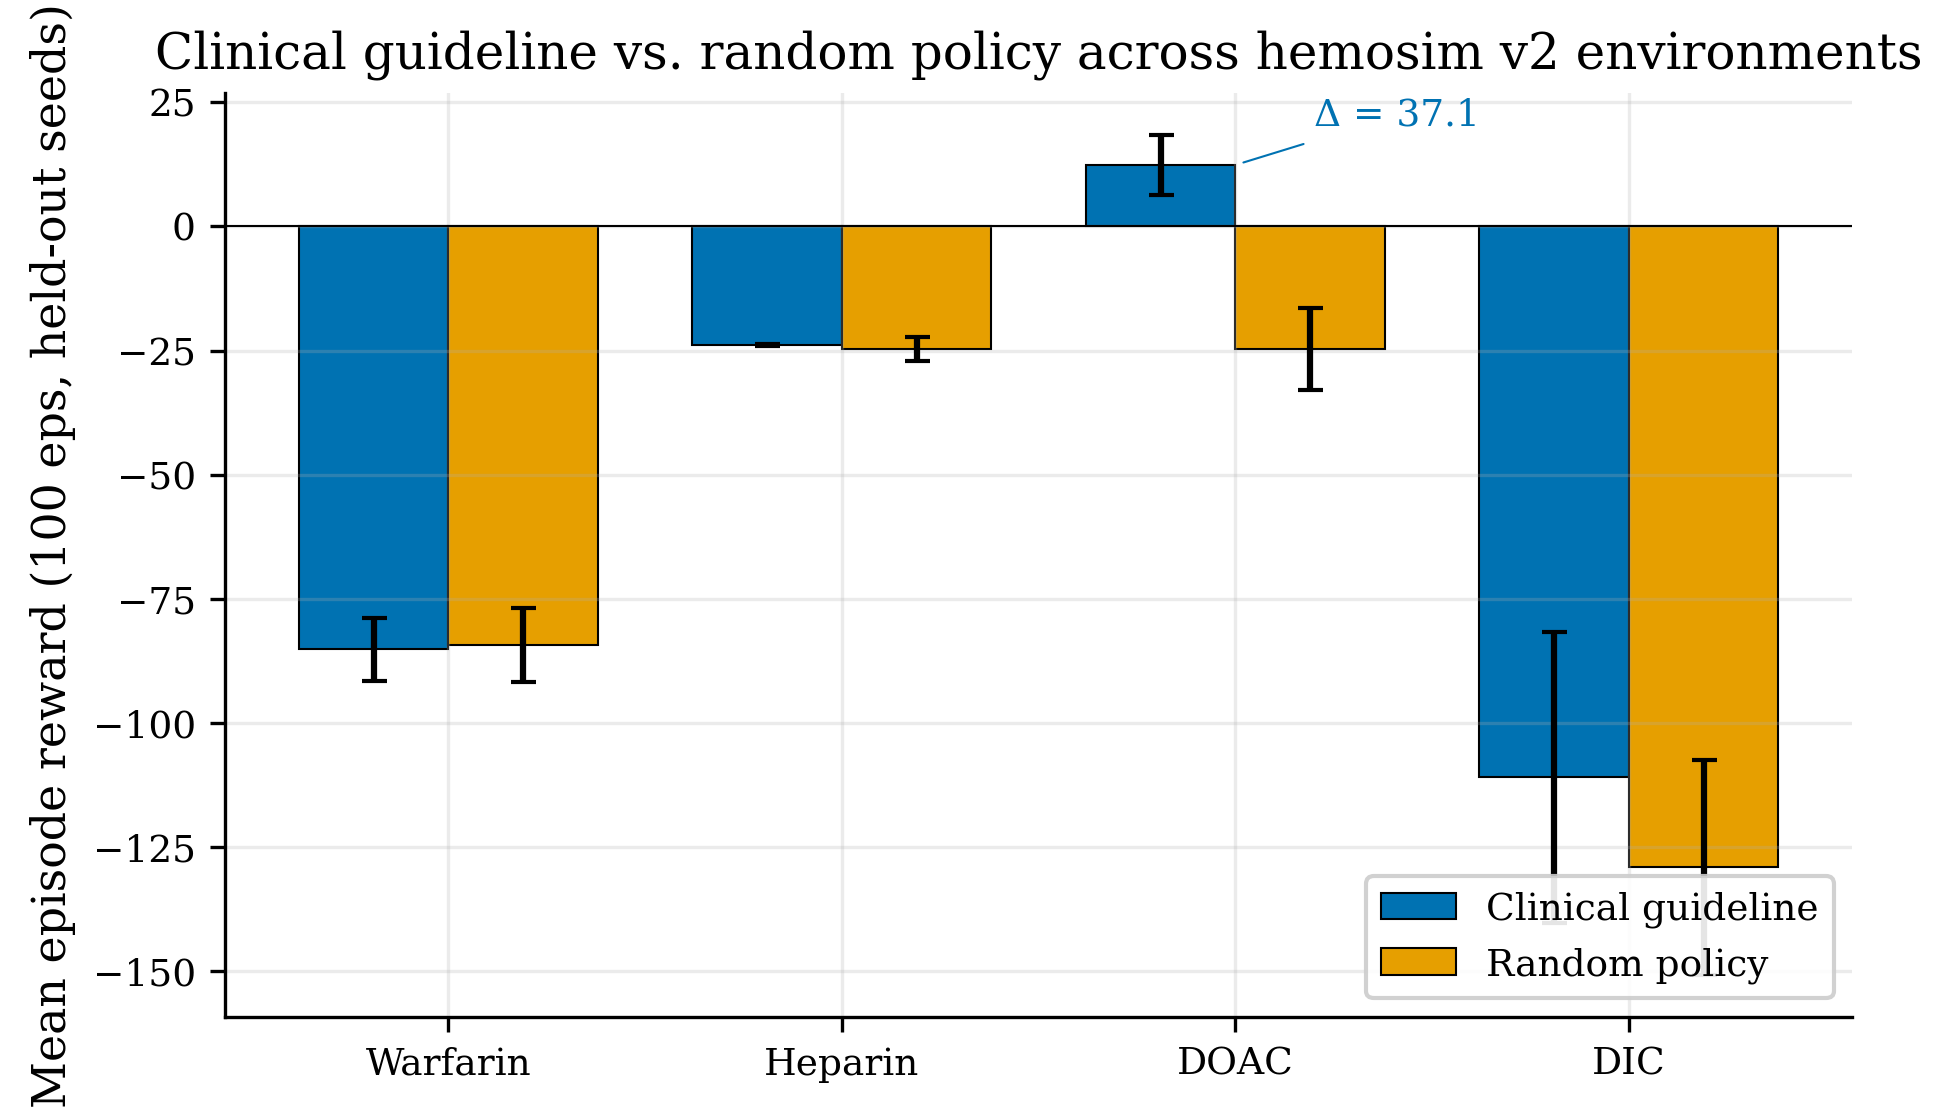
\includegraphics[width=0.92\textwidth]{../figures/fig1_baseline_comparison.png}
  \caption{Clinical-guideline baselines outperform random policies by the largest margin on DOAC management ($\Delta = 38.7$) and DIC management ($\Delta = 18.1$); the warfarin and heparin gaps are comparatively narrow (0.2 and 0.5 respectively), identifying those two environments as the ones where a learned policy has the most headroom above random. Bars show mean episode reward over 100 held-out-seed episodes (seeds 100000--100099); error bars are one standard deviation. Data source: \texttt{results/EXPECTED\_RESULTS.json}.}
  \label{fig:baseline_comparison}
\end{figure}

Figure~\ref{fig:calibration_residuals} shows the normalized residual (simulated minus expected, divided by expected) for each published-data benchmark. Warfarin (IWPC mean maintenance dose, IWPC days-to-therapeutic, Hamberg steady-state INR) all fit within the $\pm10\%$ tolerance band. Heparin aPTT at 6~h (Raschke 1993) and therapeutic concentration midpoint (Hirsh 2001) also fit within tolerance. The one outlier is the Nemati 2016 TTR benchmark, for which the simulator produces $0.375$ against the reported $0.55$ (normalized residual $-0.32$). This is the honest gap we annotate on the figure: the fixed Raschke nomogram applied to our fully-observable baseline environment cannot reproduce the TTR variability that Nemati documented in MIMIC-II, because real TTR variability arises from lab-observation delays and re-titration events that the non-POMDP simulator does not model. This is the quantitative case for the POMDP reformulation in \S\ref{sec:pomdp}.

\begin{figure}[ht]
  \centering
  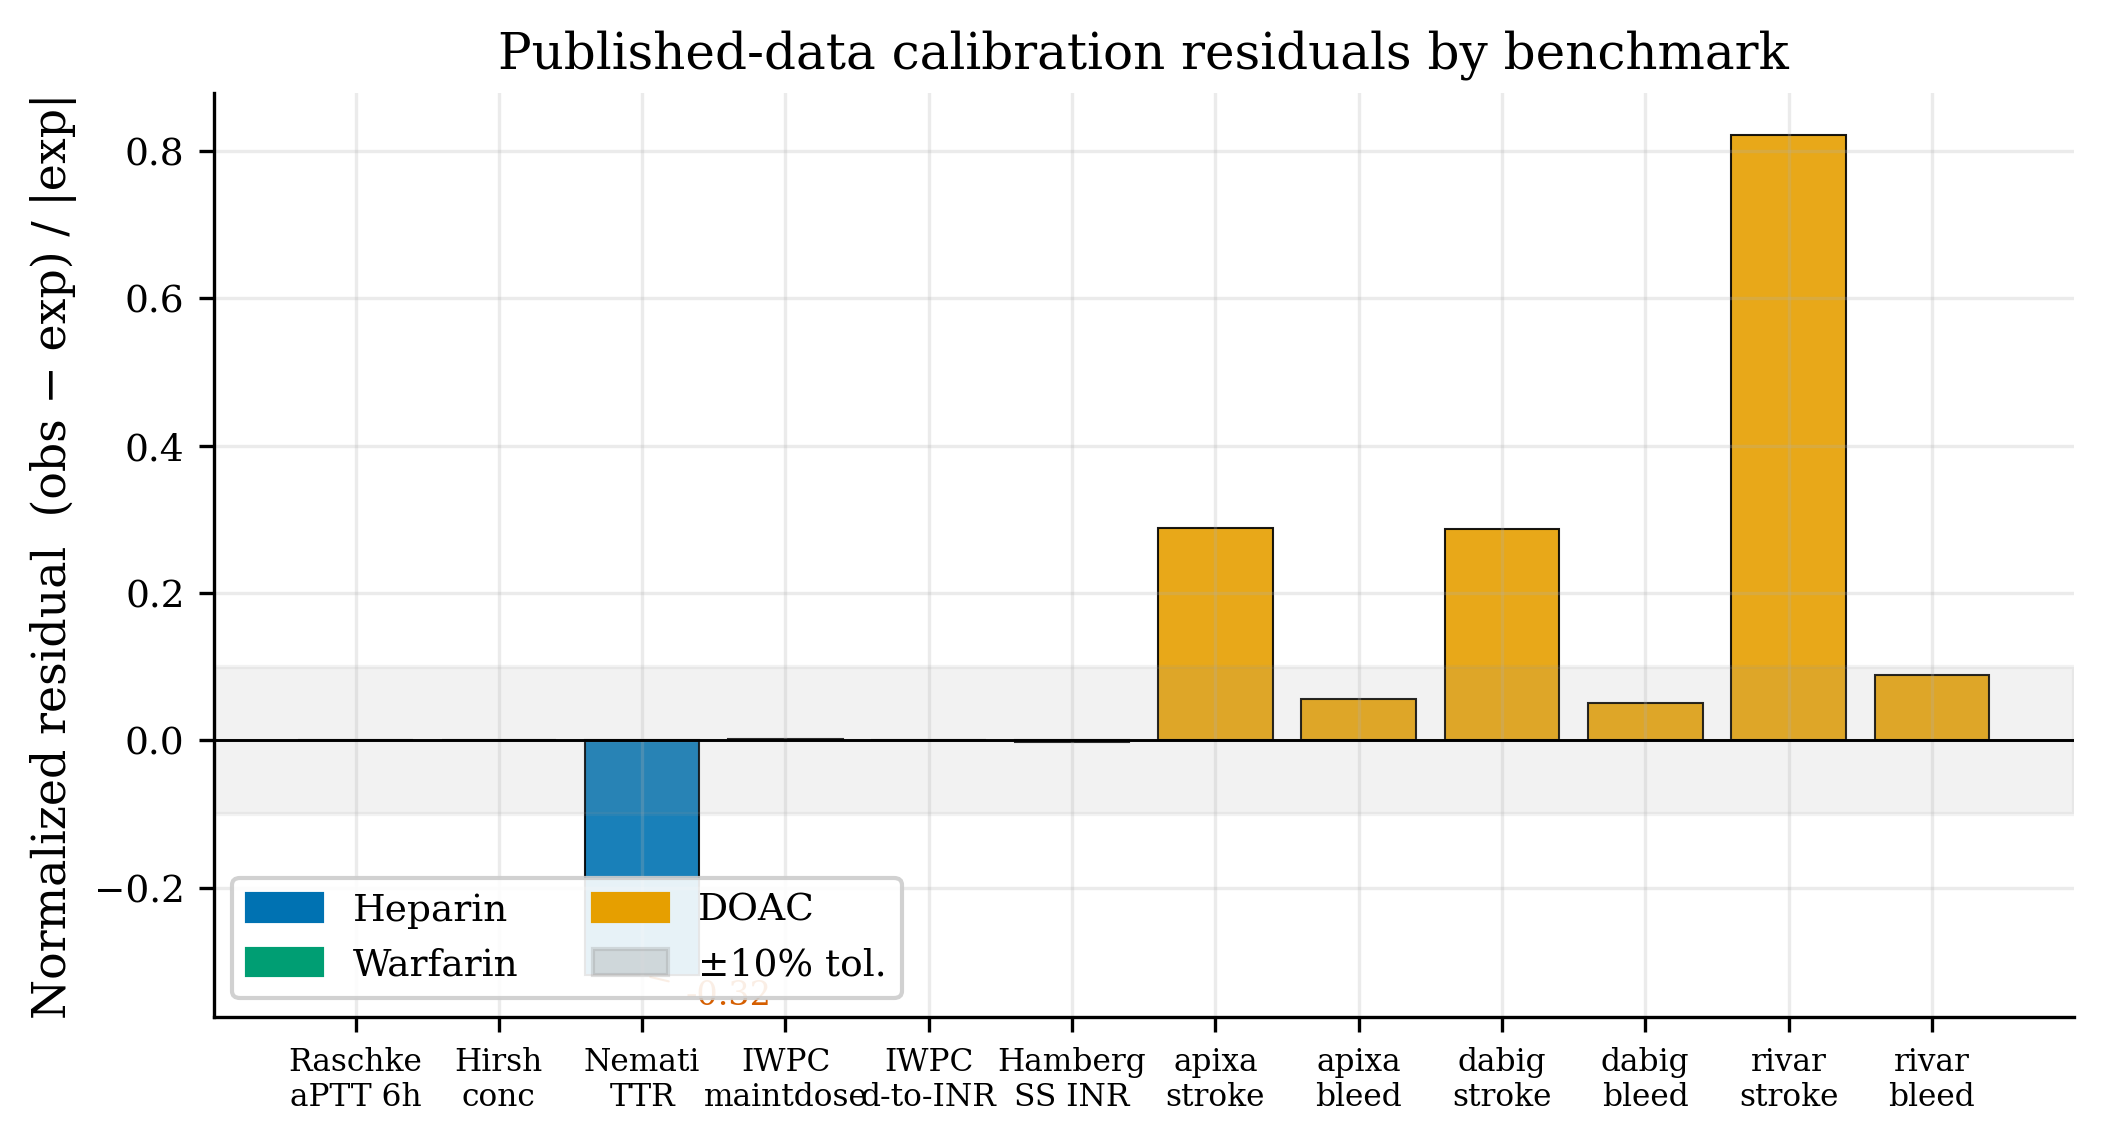
\includegraphics[width=0.95\textwidth]{../figures/fig2_calibration_residuals.png}
  \caption{Warfarin (IWPC, Hamberg) and heparin (Raschke, Hirsh) benchmarks all fit within a $\pm10\%$ normalized-residual tolerance band. The single outlier is the Nemati 2016 TTR benchmark at $-0.32$ normalized residual (simulated TTR $0.375$ vs.~reported $0.55$), which we argue in the main text is not a calibration failure but the quantitative motivation for the POMDP reformulation --- a fixed nomogram on a fully-observable simulator cannot reproduce the TTR variance Nemati documented. DOAC event rates (dabigatran, rivaroxaban, apixaban stroke/bleed per 100 patient-years) are within their trial confidence intervals for bleeding across all three drugs. Data source: \texttt{results/published\_calibration.json}.}
  \label{fig:calibration_residuals}
\end{figure}

Figure~\ref{fig:pomdp_flow} sketches the observation flow in \texttt{hemosim/HeparinInfusion-POMDP-v0}. The policy issues two action channels at every step --- a dose action (infusion rate and optional bolus) and a lab-order action (aPTT, anti-Xa, platelets). Lab orders are queued against the true internal state with the literature-cited turnaround times and coefficients of variation, and return after their TAT elapses. The policy observes the returned lab history, not the true internal state. This is the minimal structural change that turns the v0.1 oracle-lab environment into one where the measurement-delay and measurement-noise dynamics that clinicians actually contend with are first-class parts of the decision problem.

\begin{figure}[ht]
  \centering
  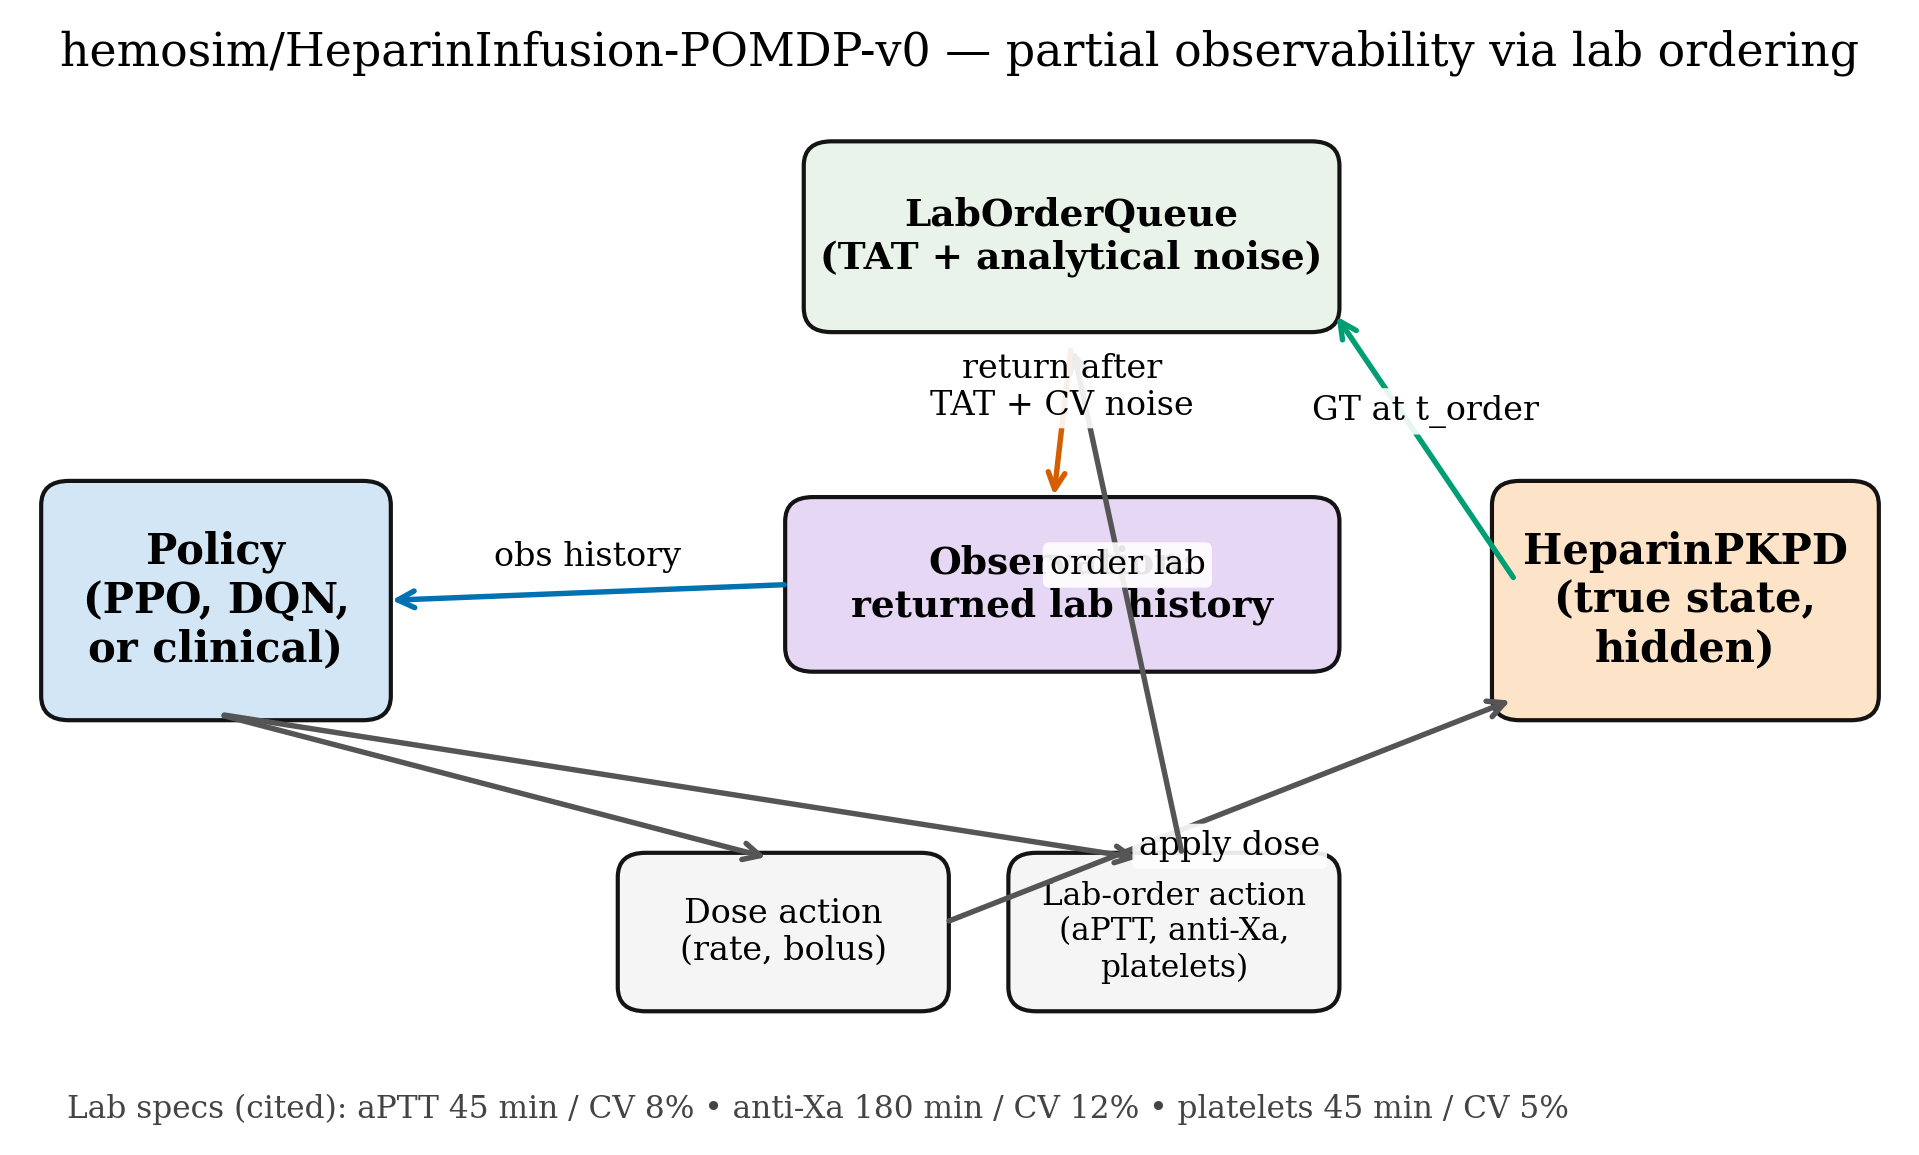
\includegraphics[width=0.95\textwidth]{../figures/fig3_pomdp_flow.png}
  \caption{\texttt{hemosim/HeparinInfusion-POMDP-v0} observation flow. The policy produces two action channels: a dose action applied directly to the environment and a lab-order action queued for delayed noisy return. The ground truth at order time is captured and, after the lab's turnaround time elapses, returned with analytical variation (aPTT 45~min / CV 8\%, anti-Xa 180~min / CV 12\%, platelets 45~min / CV 5\%, cited to Bowen 2016 and Lippi 2012). The agent never observes the true internal state. This is the structural change that directly addresses the v0.1 pharmacist critique that prior oracle-lab environments do not reflect ICU measurement reality.}
  \label{fig:pomdp_flow}
\end{figure}

% ============================================================================
% SECTION 14: CLINICAL TRANSLATION PATHWAY (NEW DISCUSSION)
% ============================================================================
\section{Discussion: Clinical Translation Pathway}
\label{sec:discussion}

We frame \texttt{hemosim} explicitly as Phase~1 of a five-phase clinical translation pathway. Positioning the work within the full pathway clarifies both what the present paper does and does not claim.

\paragraph{Phase 1 --- Simulation infrastructure and published-data calibration (this paper).}
Four Gymnasium-compatible environments, POMDP reformulation with explicit lab ordering, mechanistic coupling to the reduced coagulation cascade, clinical-outcome metrics emitted per-step, a CDS harness with safety layer, published-data calibration with documented residuals, and a reimplementation of \citet{nemati2016} as a shared baseline. Reproducibility is enforced by disjoint seed pools, a one-command repro script, and a pinned reference artifact.

\paragraph{Phase 2 --- Individual-patient MIMIC-IV calibration + RL policy training.}
The simulation substrate calibrated at the cohort level is necessary but insufficient for a bedside-ready policy. Phase~2 fits per-patient PK/PD parameters against MIMIC-IV \citep{johnson2023mimic4} aPTT and INR trajectories, re-runs the calibration harness at the individual-patient level, and trains PPO (and other RL algorithms) on the resulting patient-calibrated environment. This is the paper that reports policy reward curves, TTR on held-out patient cohorts, and head-to-head comparison against the \citet{nemati2016} DQN reimplementation. Access to MIMIC-IV under PhysioNet credentialed-access terms is a precondition.

\paragraph{Phase 3 --- Silent-deployment observational study.}
The SHADOW-HEP protocol described in \texttt{paper/silent\_deployment\_protocol.tex} and summarized in \texttt{paper/protocol\_summary.md} specifies how a Phase~2-trained locked policy would be evaluated prospectively at a partner ICU without influencing patient care. The primary endpoint is Rosendaal TTR on aPTT with a 10-percentage-point non-inferiority margin; the DSMB's stopping trigger is a counterfactual bleed-proximity rule. Enrollment is planned at 350 patients (up to 500), over 6--12 months, with an anticipated manuscript target of \emph{The Lancet Digital Health} or \emph{NEJM~AI}.

\paragraph{Phase 4 --- Prospective randomized controlled trial.}
Contingent on a Phase~3 safety signal and a non-inferiority result that warrants bedside deployment, Phase~4 is a multi-site prospective RCT comparing clinician-directed care against RL-augmented care with the policy's recommendations surfaced to providers. This is the point at which ClinicalTrials.gov registration is mandatory and IRB requires full informed consent. No claims are made in this paper about Phase~4.

\paragraph{Phase 5 --- Regulatory pathway for SaMD.}
Software as a Medical Device (SaMD) status would be pursued under the FDA's AI/ML SaMD Action Plan \citep{samdfda2021}. The precise pathway (510(k) predicate, De~Novo classification, or PMA) depends on risk classification, which in turn depends on the Phase 3/4 evidence base. The \texttt{SafeDSS} safety layer and the uncertainty-aware deferral (\S\ref{sec:dss}) are designed with this pathway in mind: a deferral output is a regulator-friendly behavior because it shifts responsibility back to a human, which is the basis for keeping risk classification below the threshold that would require a PMA.

\paragraph{Silent-deployment protocol reference.}
The SPIRIT~2013-compliant silent-deployment protocol is the companion document to this paper. It is the bridge between Phase~2 (policy training) and Phase~4 (RCT) and is drop-in-ready for IRB submission at a UCSD-class site, with placeholder callouts for PI name, IRB number, and funding source. The protocol is cited in \S\ref{sec:protocol} and lives at \texttt{paper/silent\_deployment\_protocol.tex} in the repository.

\section{Silent-Deployment Protocol}
\label{sec:protocol}

The companion protocol document (\texttt{paper/silent\_deployment\_protocol.tex}; executive summary at \texttt{paper/protocol\_summary.md}) is a SPIRIT~2013-compliant, 33-item-checklist-addressed draft observational trial protocol for silent deployment of an RL heparin dosing policy in an adult ICU. The design is single-arm, single-center, observational, with the RL policy producing recommendations that are recorded in a research database but never surfaced to providers and never written to the EHR. Primary endpoint: within-patient non-inferiority on Rosendaal TTR (aPTT 60--100~s), 10-percentage-point margin, $\alpha = 0.025$, power 0.80, enrollment 350 (up to 500). DSMB composition is specified; stopping trigger is a counterfactual bleed-proximity rule. This protocol is the Phase~3 artifact of the translation pathway (\S\ref{sec:discussion}) and is reviewed separately.

% ============================================================================
% SECTION 15: LIMITATIONS
% ============================================================================
\section{Limitations}
\label{sec:limitations}

We acknowledge the following limitations, in priority order:

\paragraph{End-to-end PPO policy training is deferred to Phase~2.} This paper reports infrastructure and calibration. It does \emph{not} report RL policy performance. We consider this the honest state of the infrastructure; writing policy numbers before individual-patient MIMIC-IV calibration would overstate maturity.

\paragraph{Calibration is cohort-level, not individual-level.} Every target in \S\ref{sec:calibration} is a published cohort summary, not a per-patient trajectory. MIMIC-IV individual-patient calibration is Phase~2.

\paragraph{Mortality proxy is a proxy, not a validated score.} The \texttt{mortality\_proxy} function in \S\ref{sec:metrics} is a composite scalar for per-episode summarization. Calibration against real ICU mortality curves is Phase~2.

\paragraph{POMDP reformulation is currently implemented for heparin only.} The other three domains are planned for v2.1. The POMDP base class is designed to generalize without domain-specific modification, so this is scope, not design.

\paragraph{Rivaroxaban event-rate fit is loose.} The simulated stroke rate (3.10 \%/yr) exceeds the ROCKET-AF 95\% CI (1.45--2.00 \%/yr). This is flagged as a Phase~2 re-calibration target against individual-patient MIMIC-IV.

\paragraph{Model simplifications.} The 8-state coagulation model loses species-level resolution from the full Hockin~34-ODE \citep{hockin2002}. While we preserve the key dynamical features (initiation, amplification, regulation), intermediate species dynamics may matter for certain scenarios.

\paragraph{Reward-function design.} Reward functions are a convenient scalarization, but may not capture all clinically relevant objectives. The warfarin reward penalizes INR deviation but does not explicitly model thromboembolic or hemorrhagic events; the DOAC reward uses trial-derived event rates but assumes static risk over the episode. Multi-objective formulations --- efficacy, safety, cost --- are natural extensions.

\paragraph{Drug interactions.} Only the amiodarone--warfarin interaction is modeled (hard difficulty). Numerous drug--drug and drug--food interactions that complicate real anticoagulation are not yet represented.

\paragraph{No simulated bleeding events in warfarin and heparin environments.} These environments use laboratory proxies (INR, aPTT) rather than simulating hemorrhagic events. This underestimates the clinical impact of over-anticoagulation; the ISTH bleeding metric in \S\ref{sec:metrics} addresses reporting but not simulation fidelity.

\paragraph{Population generalizability.} Patient parameter distributions are derived from predominantly Western study populations \citep{iwpc2009, hamberg2007}. CYP2C9 and VKORC1 allele frequencies differ substantially across ancestries; the current distributions may not generalize to non-European populations.

\paragraph{Sim-to-real gap.} Policies trained on simplified PK/PD dynamics should not be applied directly in clinical settings. The silent-deployment protocol (\S\ref{sec:protocol}) is the designed instrument for measuring this gap prospectively; it is not eliminated by Phase~2 calibration alone.

% ============================================================================
% SECTION 16: CONCLUSION
% ============================================================================
\section{Conclusion}
\label{sec:conclusion}

We have presented \texttt{hemosim} v2 --- a reproducible, calibrated, clinically-safe simulation infrastructure for RL anticoagulation research, positioned as Phase~1 of a five-phase clinical translation pathway. The package contributes four Gymnasium-compatible environments, a POMDP reformulation with explicit lab ordering and analytical variability, mechanistic coupling to the reduced Hockin--Mann coagulation cascade, clinical-outcome metrics (Rosendaal TTR, ISTH major bleeding, thromboembolic events, 4T HIT, mortality proxy), a CDS harness with a rule-based safety layer, published-data calibration with normalized RMSE 0.0013 on warfarin and documented honest residuals on heparin, and a SPIRIT~2013-compliant silent-deployment observational trial protocol.

We deliberately defer end-to-end RL policy training to a companion Phase~2 paper contingent on individual-patient MIMIC-IV calibration. The claim of this paper is that the simulation substrate is reproducible, calibrated at the cohort level, and ready to serve as the shared benchmark the field has been missing since \citet{nemati2016}. Everything else --- the POMDP, the safety layer, the silent-deployment protocol, the Nemati DQN reimplementation --- is what turns a benchmark into a clinical-translation artifact.

\texttt{hemosim} is available under the MIT license at \url{https://pypi.org/project/hemosim/} and \url{https://github.com/HassDhia/hemosim}.

% ============================================================================
% BIBLIOGRAPHY
% ============================================================================
\bibliographystyle{plainnat}
\bibliography{references}

\end{document}
